\section{Introduction}
\label{sec:intro}
Large Language Models (LLMs)~\cite{chatgpt2025, comanici2025gemini} have been increasingly deployed into autonomous agents to tackle complex tasks~\cite{mialon2023gaia,yang2024swe,zheng2024gpt}. Such capability emerges from the orchestration of long-horizon planning, multi-hop retrieval, iterative tool use, dynamic reasoning and human-in-the-loop interaction. 

However, hallucination, the generation of plausible yet non-factual content, remains a persistent issue in LLM-based systems. Unlike LLM hallucinations confined to single-turn responses~\cite{huang2025survey,ji2023survey}, agent-based hallucinations are amplified by the sequential nature of multi-step workflows, where intermediate errors propagate and ultimately degrade the final response~\cite{zhou2025guardian}. As shown in Figure~\ref{fig:example_illus} \textbf{Left}, a planning hallucination misdefines ``region X, Y, Z'', which propagates into downstream Python tool parameters and leads to an incorrect final answer. This underscores an urgent need for granular analyses to pinpoint the origin of the hallucination, especially in high-stakes agentic applications~\cite{huang2025survey}. 

% \xiao{This paragraph should emphasize a brief definition of hallucination, its unique characteristics and urgency. e.g., agent hallucinations, the generation of plausible but factually incorrect information, pose a critical threat to the reliability and safety of such systems. Unlike single-turn LLM responses where errors remain localized, agent workflows operate through sequential multi-step reasoning, where a hallucination at any intermediate step can propagate through subsequent actions, compound over time, and ultimately lead to catastrophically wrong outcomes. As illustrated in Fig. 1 (Left), XXX. In high-stakes domains such as XXX, underscoring the urgent need to understand \textbf{where} and \textbf{why} hallucinations originate in agentic workflows.}

% \xiao{In the next paragraph, how do existing methods work? What are their limitations? What are the tasks we need to accomplish, and what challenges do they present? e.g., existing approaches to hallucination detection predominantly focus on binary judgment—determining whether a given output is hallucinated or factual[][][]. While valuable, these methods treat the entire response as an atomic unit and operate exclusively on single-turn outputs, fundamentally limiting their applicability to agentic systems. This binary paradigm fails to address several critical questions essential for building reliable agents: (1) Which specific step in the trajectory first introduced the hallucination? (2) What was the causal mechanism that triggered the error? XXX}

\begin{figure}[!t]
  \centering
    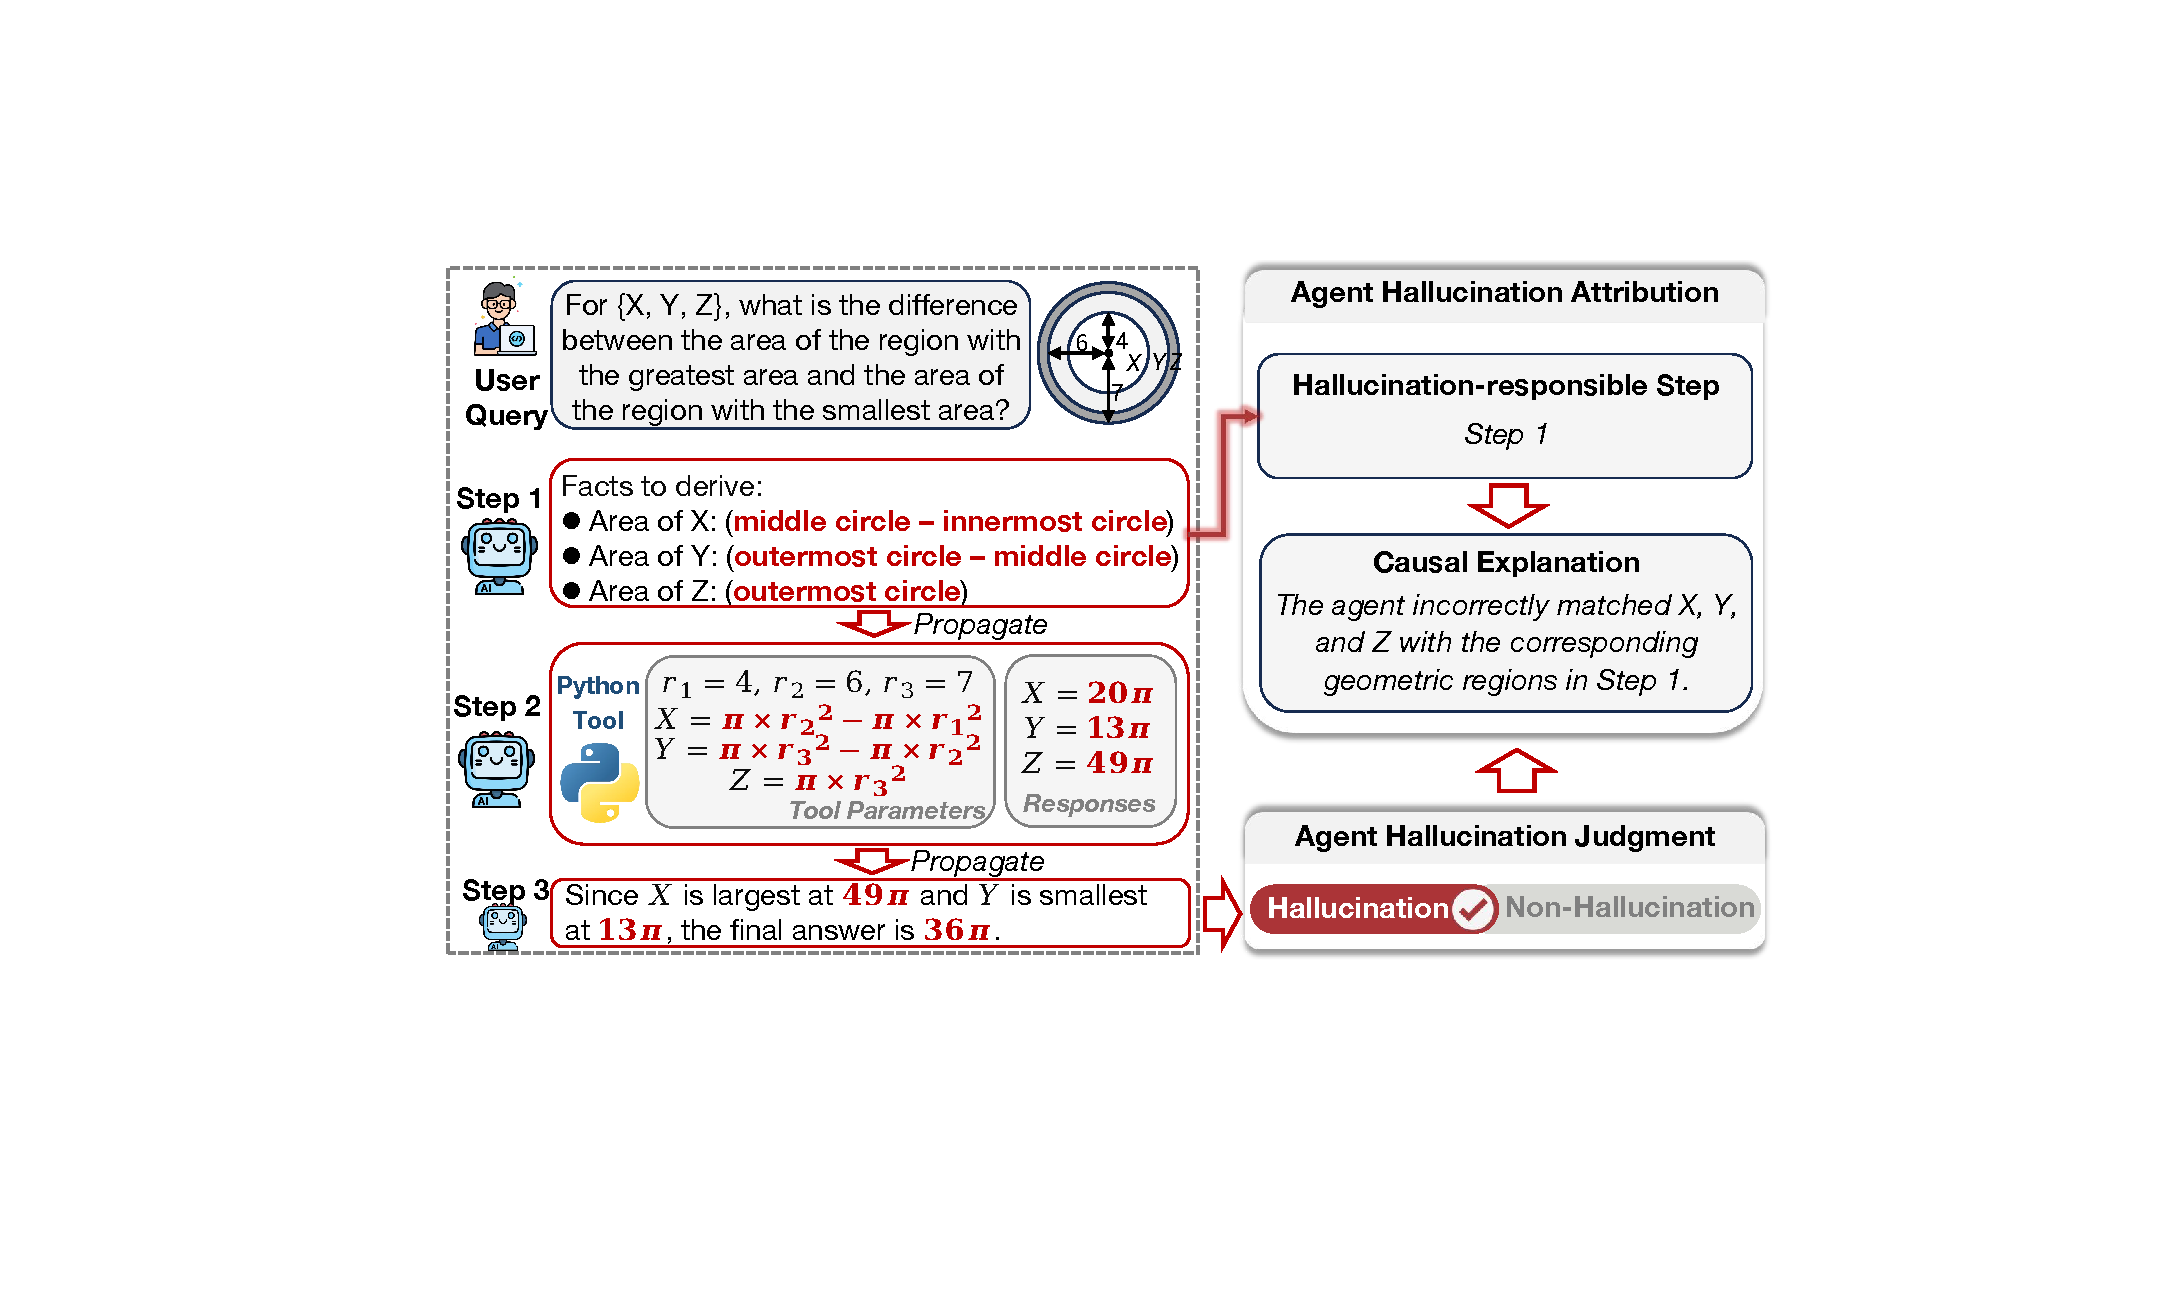
\includegraphics[width=1.0\linewidth]{Fig/figure1.pdf}
    % \vspace{-1.8em}
    \caption{ Illustration of hallucination attribution in LLM-based agents. \textbf{Left:} A misdefinition of regions X, Y, Z in Step 1 propagates to the tool call and leads to the incorrect final answer. \textbf{Right:} Beyond binary judgment, hallucination attribution aims to identify a hallucination-responsible step and a causal explanation.
    }
    \label{fig:example_illus}
\end{figure}

\begin{table*}[t]
    \centering
    \tabcolsep=5pt
    \caption{Comparison of AgentHallu with existing hallucination detection datasets in terms of dataset statistics (sample size (\textbf{\#Samp.}) and trajectory steps (\textbf{\#Step})), hallucination categories (planning hallucination (\textbf{Planning}), retrieval hallucination (\textbf{Retrieval}), reasoning hallucination (\textbf{Reasoning}), human-interaction hallucination (\textbf{Human}), and tool-use hallucination (\textbf{Tool})), and task type (Hallucination \textbf{Judgment} and Hallucination \textbf{Attribution}).
}
       \vspace{-0.8em}
    \label{dataset_comparison}
    \resizebox{\linewidth}{!}{
    % \tablestyle{4.5pt}{1.10}
\begin{tabular}{l|cc|ccccc|cc}
\toprule
\multirow{2}{*}{\textbf{Dataset}} & \multicolumn{2}{c|}{\textbf{Dataset Statistic}} & \multicolumn{5}{c|}{\textbf{Hallucination Category}}         & \multicolumn{2}{c}{\textbf{Task Type}} \\ \cline{2-10} 
                         & \textbf{\#Samp.}        & \textbf{\#Step}        & \textbf{Planning} & \textbf{Retrieval} & \textbf{Reasoning} & \textbf{Human} & \textbf{Tool} & \textbf{Judgment}     & \textbf{Attribution}    \\ \midrule \midrule
HaluEval~\cite{li2023halueval}                 & 35,000         & 1             & \crossmark     & \crossmark      & \checkmark      & \crossmark  & \crossmark & \checkmark         & \crossmark           \\
FELM~\cite{zhao2023felm}                     & 847            & 1             & \crossmark     & \crossmark      & \checkmark      & \crossmark  & \crossmark & \checkmark         & \crossmark           \\
SAC$^3$~\cite{zhang2023sac3}                     & 500            & 1             & \crossmark     & \crossmark      & \checkmark      & \crossmark  & \crossmark & \checkmark         & \crossmark           \\
FAVABench~\cite{mishra2024fine}                & 902            & 1             & \crossmark     & \crossmark      & \checkmark      & \crossmark  & \crossmark & \checkmark         & \crossmark           \\
RAGTruth~\cite{niu2024ragtruth}                 & 2,965          & 1             & \crossmark     & \checkmark      & \crossmark      & \crossmark  & \crossmark & \checkmark         & \crossmark           \\
ToolBH~\cite{zhang2024toolbehonest}                   & 700            & 1             & \crossmark     & \crossmark      & \crossmark      & \crossmark  & \checkmark & \checkmark         & \crossmark           \\
\midrule
\rowcolor{LightCyan}
\textbf{AgentHallu (Ours)}        & 693            & 7.6           & \checkmark     & \checkmark      & \checkmark      & \checkmark  & \checkmark & \checkmark         & \checkmark           \\ \bottomrule
\end{tabular}
    }
\end{table*}



















Current hallucination evaluations~\cite{bang2025hallulens,niu2024ragtruth,li2023halueval} primarily classify single-turn LLM responses as factual or hallucinated. While valuable, this binary paradigm fails to address concerns essential for building reliable agents: \textbf{where} and \textbf{why} hallucinations originate in agentic workflows. To fill this gap, we propose a novel research task of \textbf{automated hallucination attribution} for LLM-based agents. We define two key objectives: \textbf{(1) Hallucination-responsible Step Localization (Where):} identify the step responsible for the hallucinated result, (2) \textbf{Causal Explanation (Why):} provide an open-ended explanation of the underlying cause. As shown in Figure~\ref{fig:example_illus} \textbf{Right}, step attribution precisely identifies ``Step 1'' as the hallucination origin, while causal explanation provides a corresponding diagnostic analysis of ``Step 1 incorrectly matched X, Y, and Z with their regions''.

To support this task, we present AgentHallu, the first comprehensive benchmark tailored for automated hallucination attribution of multi-step agent trajectories. As shown in Table~\ref{dataset_comparison}, the key highlights of the AgentHallu dataset include: \textit{(1) Extensive Diversity.} We collect 693 trajectories from 7 popular agent frameworks with an average length of 7.6 steps. The dataset encompasses five distinct domains: world knowledge, science, math, general assistant, and tool use. \textit{(2) High-quality Control.} We implement a rigorous three-stage filtering criterion to exclude non-deceive failures, overly short sequences, and trivial cases lacking diagnostic depth, thereby ensuring the benchmark's difficulty. \textit{(3) Comprehensive Taxonomy.} We develop a hierarchical taxonomy of agent hallucinations via grounded theory~\cite{glaser2017discovery}, resulting in 5 primary categories (Planning, Retrieval, Reasoning, Human-Interaction, and Tool-Use) and 14 granular subcategories. \textit{(4) Multi-level Annotation.} AgentHallu includes binary labels for judgment. For attribution, it specifies hallucination-responsible steps and explains the underlying cause in plain language. All annotations are manually curated through a labor-intensive process.

% \begin{itemize}[noitemsep,left=2pt, itemsep=0pt, topsep=0pt]
%     \item \textit{Extensive Diversity}. We collect 693 trajectories from 7 popular agent frameworks with an average length of 7.6 steps. The dataset encompasses five distinct domains: world knowledge, science, math, general assistant, and tool use.
%     \item \textit{High-quality Control}. We implement a rigorous three-stage filtering criterion to exclude non-deceive failures, overly short sequences, and trivial cases lacking diagnostic depth, thereby ensuring the benchmark's difficulty.
%     \item \textit{Comprehensive Taxonomy}. We develop a hierarchical taxonomy of agent hallucinations via grounded theory~\cite{glaser2017discovery}, resulting in 5 primary categories (Planning, Retrieval, Reasoning, Human-Interaction, and Tool-Use) and 14 granular subcategories.
%     \item \textit{Multi-level Annotation}. AgentHallu includes binary labels suitable for judgment. For attribution, it specifies hallucination-responsible steps and explains the underlying cause in plain language.
% \end{itemize}


% \textbf{Dataset.} AgentHallu comprises 693 high-quality trajectories annotated trajectories designed to facilitate automated hallucination attribution. AgentHallu offers several key advantages. (1) Extensive Diversity. We collect trajectories from 7 popular agent frameworks, spanning five distinct domains: world knowledge, science, math, general assistant, and tool use. (2) Comprehensive Taxonomy. We develop a hierarchical taxonomy of agent hallucinations via grounded theory, resulting in 5 primary categories (Planning, Retrieval, Reasoning, Human-Interaction, and Tool-Use) and 14 granular subcategories. (3) High-quality Control. We implement a rigorous three-stage filtering criterion to exclude non-deceive failures, overly short sequences, and trivial cases lacking diagnostic depth, thereby ensuring the benchmark's difficulty. (4) Fine-grained Annotation. Each trajectory is meticulously annotated with binary labels, step-wise localization, granular categories, and explainable cause.

% \textbf{Metric.} Rather than relying solely on binary judgment metrics, AgentHallu supports attribution evaluation via two metrics: step-level localization accuracy for identifying the decisive step, and G-EVAL scores for assessing the quality of open-ended rationales. This approach provides deeper insights into the agent's underlying failure mechanisms and identifies areas for improvement beyond simple outcome correctness.

Using the AgentHallu, we develop an attribution evaluation framework along two dimensions: step localization accuracy as a measure of responsible-step identification, and G-EVAL scores~\cite{liu2023g} for assessing the quality of open-ended explanations. Leveraging this framework, we evaluate 13 leading LLMs, including 5 proprietary and 8 open-source models. Empirical results reveal several critical findings: (1) The best-performing model, Gemini-2.5-Pro, achieves only 41.1\% accuracy in step localization, which drops to 11.6\% accuracy on tool-use hallucinations. (2) Step-by-Step prompting improves attribution via incremental processing, but at the cost of higher token usage. (3) Increasing trajectory steps $N_{\text{step}}$ poses a challenge to attribution, with GPT-5's accuracy dropping from 40.3\% ($N_{\text{step}} \le 5$) to 23.9\% ($N_{\text{step}} \ge 11$).

% Increasing trajectory steps poses a significant challenge to attribution, with GPT-5's accuracy dropping from 29.9\% ($N_{\text{step}} \le 5$) to 11.4\% ($N_{\text{step}} \ge 11$).

% Increased trajectory steps poses a significant challenge to attribution, due to accumulated distracting context.


% In contrast, open-source models achieve extremely low performance with 10.7\% accuracy on average, only marginally above a random baseline of 8.7\%.

Overall, our contributions include: (i) A novel task of automated hallucination attribution in LLM-based agents to understand where and why hallucinations originate. (ii) A comprehensive benchmark comprising 693 high-quality trajectories with broad diversity, a systematic taxonomy and multi-level annotations. (iii) Evaluation of 13 leading LLMs, revealing their strengths and limitations under varying conditions, including hallucination categories, prompting methods, and trajectory steps.


